On behalf of the Organizing Committee and the Technical Program Committee,
we are delighted to welcome you to the \textbf{4th IEEE International Conference on Power Electronics, Smart Grid, and Renewable Energy (IEEE PESGRE 2025)}, hosted at the vibrant campus of Indian Institute of Technology Dharwad, Karnataka, India, from December 18 - 21, 2025.

IEEE PESGRE is the biennial flagship conference of \textbf{IEEE Kerala Section, IEEE IA/IE/PELS Joint Chapter Kerala}, and the \textbf{IEEE Industry Applications Society}, with financial co-sponsorship from these bodies. Technical co-sponsors include the \textbf{IEEE Power Electronics Society}, \textbf{IEEE Industrial Electronics Society}, and \textbf{IEEE Power \& Energy Society}.

The theme for this edition is \textbf{``Power Electronics and Renewable Energy for Sustainable Development }. The conference will spotlight cutting-edge technologies, strategies, and challenges in power electronics, renewable energy, electric vehicles, grid integration, and smart grid solutions. IEEE PESGRE 2025 serves as a global platform for exchanging ideas, presenting technical innovations, and discussing current trends and future perspectives in areas such as power converter topology, control techniques, grid integration, etc.

This edition conference reflects a truly international scope, with participants and presentations from \textbf{15 countries}, which includes, Canada, China, Estonia, Germany, India, Israel, Italy, Norway, the Netherlands, New Zealand, Poland, UAE, USA, etc. This shows the increasing popularity of the conference by underscoring the global commitment to advancing energy systems.

Out of \textbf{400 submissions, 210 papers} were accepted after a rigorous review process with three reviewers per paper involving \textbf{20 track chairs} and \textbf{350 expert reviewers} from different countries.  Finally, a total of \textbf{179 camera-ready papers} will be presented across 30 technical oral sessions.
%
The program features:
%
%\parbox{\linewidth}{
\begin{itemize}
\setlength{\itemsep}{0pt}        % Space between items
\setlength{\parskip}{0pt}        % Space between paragraphs within an item
\setlength{\parsep}{0pt}         % Additional paragraph separation
\item 4 Keynote Addresses
\item 1 IES SYPA Keynote
\item 4 Tutorials
\item Two Women in Engineering (WiE) Sessions
\item PELS Young Professional Mentorship Program
\item Panel Discussion
\item Five Industry Sessions
\item Three oral presentation sessions covering 180 papers and 
\item Cultural events 
\end{itemize}
%}

We are proud to note the strong industry presence at PESGRE 2025, highlighting the growing real-world relevance of power electronic technologies and the importance of academia-industry collaboration. Together, we are shaping the future of sustainable energy systems. This belief is strengthened by our sponsors who are from different industrial sectors, related to manufacturers of power supplies and testing equipment, defence systems, renewable energy, battery technology, simulation tools, etc. 
Our sincere appreciation goes to the sponsors for their invaluable support:
\begin{itemize}
\setlength{\itemsep}{0pt}        % Space between items
\setlength{\parskip}{0pt}        % Space between paragraphs within an item
\setlength{\parsep}{0pt}         % Additional paragraph separation
	\item \textbf{Title Sponsor}: JSCGI Private Limited
	\item \textbf{Platinum Sponsors}: Pragna Microdesigns and Defence Research and Development Organisation (DRDO)
	\item \textbf{Gold Sponsors}: Convergent Technologies + Tektronix
	\item \textbf{Silver Sponsors}: Karnataka Renewable Energy Development Limited (KREDL), OPAL-RT Technologies, and AARJAY International
	\item \textbf{Bronze Sponsors}: Charge House, HIOKI, Typhoon HIL, MathWorks, CDAC, and COMSOL
	\item \textbf{Other Sponsors}: Amara Raja Group, IFB, Reliamotive Labs, FLUKE, and Keysight
\end{itemize}



We extend our heartfelt gratitude to the Technical Program Committee chairs, track chairs, and reviewers for ensuring the high technical quality of this event, and to the authors, whose innovative contributions form the core of this conference.
Finally, as we gather to share knowledge and explore innovations, let us remember our common mission: building resilient, efficient, and sustainable energy systems. Power electronic technologies are at the heart of this transformation, and your participation is vital in shaping the future.
We encourage you to take full advantage of networking opportunities—during technical sessions, coffee breaks, and social events. 
We look forward to having you all here and have an inspiring, productive, and memorable week in Dharwad.

\vspace{-2mm}
\begin{center}
	\begin{tabular}{ccccc}
		\centering
		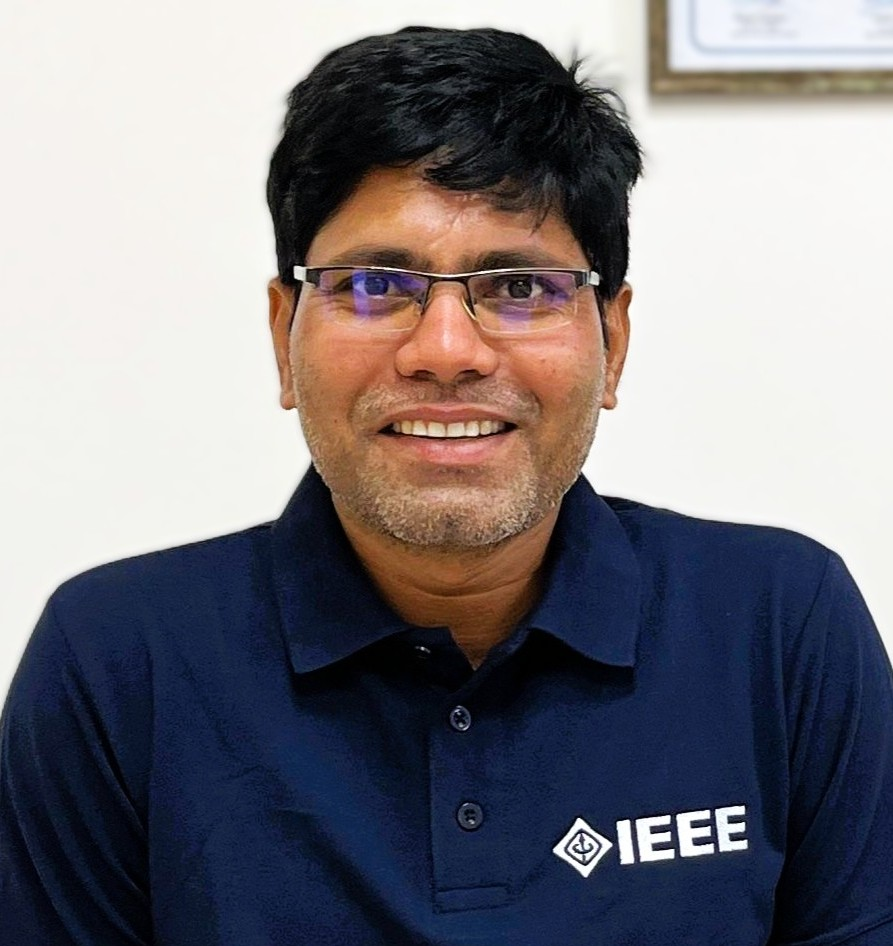
\includegraphics[width=35mm]{images/gc_satish.jpg} & \hspace{10mm}
		& 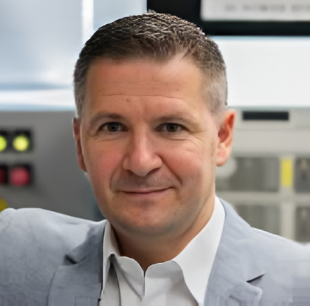
\includegraphics[width=35mm]{images/gc_dimitri.png} & \hspace{5mm}
		&  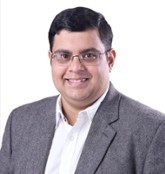
\includegraphics[width=35mm]{images/gc_sheldon.jpeg}\\
		Dr. Satish Naik & \hspace{10mm}
		& Dr. Dmitri Vinnikov & \hspace{10mm}
		&  Dr. Sheldon Williamson\\
		& & & & \\
		\multicolumn{5}{c}{Co-General Chairs, IEEE PESGRE 2025}
	\end{tabular}
\end{center}
